\documentclass[tikz,border=10pt]{standalone}
\usepackage{tikz}
\usetikzlibrary{arrows.meta,positioning,calc,backgrounds,fit,shapes.geometric}
\usepackage[scaled=0.92]{helvet}
\renewcommand{\familydefault}{\sfdefault}
\usepackage{amsmath,amssymb}
\definecolor{ink}{HTML}{262624}
\definecolor{mute}{HTML}{8A8984}
\definecolor{line}{HTML}{BDBBB5}
\definecolor{acc}{HTML}{2A78D6}
\definecolor{accbg}{HTML}{F1F6FD}
\tikzset{
  >={Latex[length=2.2mm]},
  every node/.style={text=ink},
  b/.style={draw=line, fill=white, rounded corners=2pt, align=center, inner sep=6pt,
            minimum height=10mm, text width=#1, font=\small},
  b/.default=40mm,
  a/.style={b=#1, draw=acc, fill=accbg},
  a/.default=40mm,
  t/.style={font=\footnotesize, text=mute, align=center},
  e/.style={->, draw=mute, line width=0.6pt},
  ea/.style={->, draw=acc, line width=0.9pt},
  eh/.style={->, draw=acc, line width=0.9pt, dash pattern=on 3pt off 2pt},
}

\definecolor{brn}{HTML}{B5651D}
\begin{document}
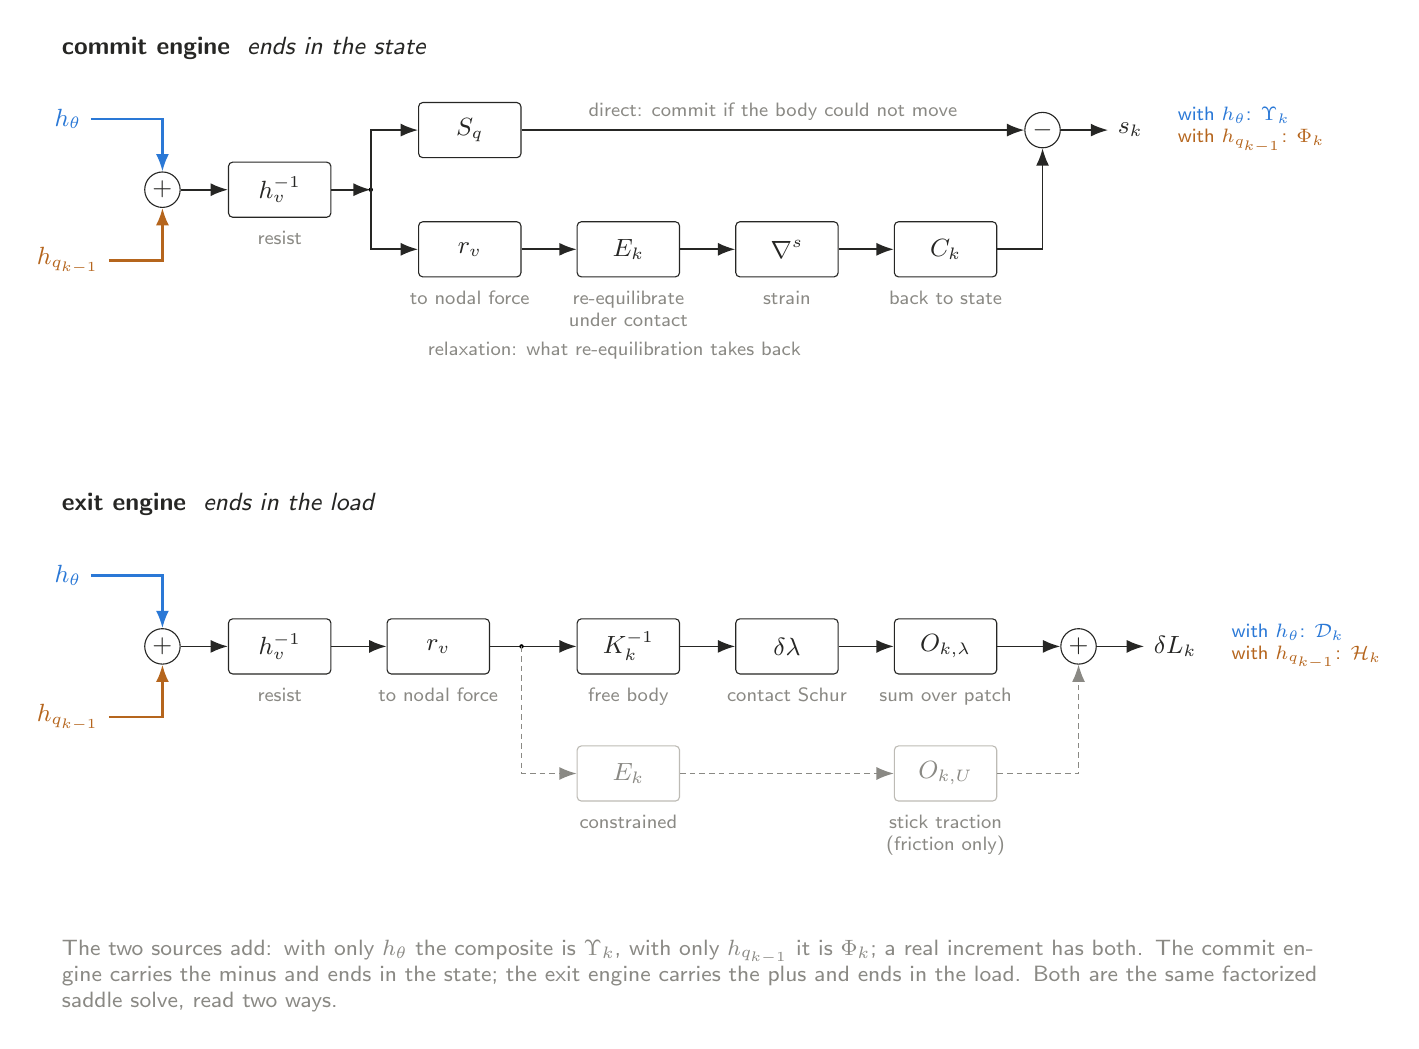
\begin{tikzpicture}
\tikzset{
  op/.style={draw=ink, fill=white, rounded corners=1.5pt, minimum width=13mm, minimum height=7mm, font=\small},
  opg/.style={op, draw=line, text=mute},
  sum/.style={circle, draw=ink, fill=white, inner sep=0pt, minimum size=4.5mm, font=\small},
  w/.style={->, draw=ink, line width=0.6pt},
  wg/.style={->, draw=mute, line width=0.5pt, dash pattern=on 2pt off 1.5pt},
  lb/.style={font=\scriptsize, text=mute, align=center},
}
% ---------- commit engine ----------
\node[anchor=west, font=\small] at (0,0) {\textbf{commit engine}\ \ {\itshape ends in the state}};
\node[font=\small, text=acc] (a1) at (2mm,-9mm) {$h_\theta$};
\node[font=\small, text=brn] (b1) at (2mm,-27mm) {$h_{q_{k-1}}$};
\node[sum] (S1) at (14mm,-18mm) {$+$};
\draw[->, acc, line width=0.8pt] (a1) -| (S1); \draw[->, brn, line width=0.8pt] (b1) -| (S1);
\node[op, right=6mm of S1] (hv) {$h_v^{-1}$}; \node[lb, below=0.5mm of hv] {resist};
\coordinate[right=5mm of hv] (J);
\node[op, above right=4mm and 6mm of J] (Sq) {$S_q$};
\node[op, below right=4mm and 6mm of J] (rv) {$r_v$}; \node[lb, below=0.5mm of rv] {to nodal force};
\node[op, right=7mm of rv] (E) {$E_k$}; \node[lb, below=0.5mm of E] {re-equilibrate\\ under contact};
\node[op, right=7mm of E] (gs) {$\nabla^s$}; \node[lb, below=0.5mm of gs] {strain};
\node[op, right=7mm of gs] (Ck) {$C_k$}; \node[lb, below=0.5mm of Ck] {back to state};
\node[sum, right=10mm of Ck |- Sq] (M) {$-$};
\node[font=\small, right=6mm of M] (s) {$s_k$};
\draw[w] (S1) -- (hv); \draw[w] (hv) -- (J); \fill (J) circle (0.8pt);
\draw[w] (J) |- (Sq); \draw[w] (J) |- (rv);
\draw[w] (rv) -- (E); \draw[w] (E) -- (gs); \draw[w] (gs) -- (Ck); \draw[w] (Ck) -| (M);
\draw[w] (Sq) -- node[above, lb]{direct: commit if the body could not move} (M); \draw[w] (M) -- (s);
\node[anchor=west, font=\scriptsize, align=left] at ($(s.east)+(2mm,0)$) {\color{acc}with $h_\theta$: $\Upsilon_k$\\ \color{brn}with $h_{q_{k-1}}$: $\Phi_k$};
\node[lb, anchor=north west] at ($(rv.south west)+(0,-7mm)$) {relaxation: what re-equilibration takes back};
% ---------- exit engine ----------
\begin{scope}[shift={(0,-58mm)}]
\node[anchor=west, font=\small] at (0,0) {\textbf{exit engine}\ \ {\itshape ends in the load}};
\node[font=\small, text=acc] (a2) at (2mm,-9mm) {$h_\theta$};
\node[font=\small, text=brn] (b2) at (2mm,-27mm) {$h_{q_{k-1}}$};
\node[sum] (S2) at (14mm,-18mm) {$+$};
\draw[->, acc, line width=0.8pt] (a2) -| (S2); \draw[->, brn, line width=0.8pt] (b2) -| (S2);
\node[op, right=6mm of S2] (hv2) {$h_v^{-1}$}; \node[lb, below=0.5mm of hv2] {resist};
\node[op, right=7mm of hv2] (rv2) {$r_v$}; \node[lb, below=0.5mm of rv2] {to nodal force};
\coordinate[right=4mm of rv2] (J2);
\node[op, right=7mm of J2] (Ki) {$K_k^{-1}$}; \node[lb, below=0.5mm of Ki] {free body};
\node[op, right=7mm of Ki] (dl) {$\delta\lambda$}; \node[lb, below=0.5mm of dl] {contact Schur};
\node[op, right=7mm of dl] (O) {$O_{k,\lambda}$}; \node[lb, below=0.5mm of O] {sum over patch};
\node[sum, right=8mm of O] (P2) {$+$};
\node[font=\small, right=6mm of P2] (L) {$\delta L_k$};
\draw[w] (S2) -- (hv2); \draw[w] (hv2) -- (rv2); \draw[w] (rv2) -- (Ki); \fill (J2) circle (0.8pt);
\draw[w] (Ki) -- (dl); \draw[w] (dl) -- (O); \draw[w] (O) -- (P2); \draw[w] (P2) -- (L);
\node[opg, below=9mm of Ki] (E2) {$E_k$}; \node[lb, below=0.5mm of E2] {constrained};
\node[opg, below=9mm of O] (OU) {$O_{k,U}$}; \node[lb, below=0.5mm of OU] {stick traction\\ (friction only)};
\draw[wg] (J2) |- (E2); \draw[wg] (E2) -- (OU); \draw[wg] (OU) -| (P2);
\node[anchor=west, font=\scriptsize, align=left] at ($(L.east)+(2mm,0)$) {\color{acc}with $h_\theta$: $\mathcal D_k$\\ \color{brn}with $h_{q_{k-1}}$: $\mathcal H_k$};
\end{scope}
\node[t, anchor=north west, align=left, text width=160mm] at (0,-112mm) {The two sources add: with only $h_\theta$ the composite is $\Upsilon_k$, with only $h_{q_{k-1}}$ it is $\Phi_k$; a real increment has both. The commit engine carries the minus and ends in the state; the exit engine carries the plus and ends in the load. Both are the same factorized saddle solve, read two ways.};
\end{tikzpicture}
\end{document}
